\chapter{Implementasi dan Pengujian}

Bab ini akan membahas seluruh proses implementasi yang dilakukan untuk menerapkan rancangan yang sudah didefinisikan sebelumnya. Selain itu, bab ini juga akan membahas pengujian yang dilakukan terhadap hasil implementasi yang mencakup hal-hal yang diuji, metode pengujian, dan hasil pengujian yang diperoleh. 


\section{Implementasi}
Implementasi sistem \textit{Performance Regression Analysis} (PRA) akan dibuat berdasarkan rancangan arsitektur seperti yang terdapat pada gambar \ref{arch-pra}. Komponen seperti \textit{library} instrumentasi, melainkan akan melakukan \textit{fork} dan modifikasi solusi \textit{Open Source} \textit{distributed tracing} dari Zipkin. Komponen yang akan dibuat dari awal sepenuhnya adalah komponen PRA \textit{User Interface} (UI) dan PRA Engine dari sistem PRA yang akan melakukan komputasi utama sistem pendeteksian dan analisis regresi. Komponen PRA Engine juga akan berfungsi sebagai API yang akan diakses oleh komponen PRA UI.



\subsection{Implementasi \textit{Performance Regression Analysis} \textit{engine}}

Sebelum melakukan implementasi solusi, penulis harus terlebih dahulu melakukan pemilihan kakas yang akan digunakan melakukan implementasinya. Secara umum, terdapat banyak bahasa pemrograman yang dapat melakukan implementasi solusi komponeasdn \textit{engine} sesuai dengan alur yang terdapat pada gambar \ref{alur-pra}. Namun, ada suatu kebutuhan penting untuk melakukan tes statistik Kolmogorov-Smirnov (K-S) yang tidak semua bahasa pemrograman memiliki dukungan \textit{library} untuk melakukannya. Terdapat dua bahasa pemrograman yang memiliki \textit{library} untuk melakukan tes K-S yaitu bahasa pemrograman \textbf{Go} dan \textbf{Python}. Bahasa \textbf{Go} memiliki library Gonum \footnote{\url{gonum.org}} yang memiliki implementasi tes K-S dalam fungsi \texttt{KolmogorovSmirnov}, sementara bahasa \textbf{Python} memiliki library SciPy \footnote{\url{scipy.org}} yang memiliki implementasi tes K-S dalam fungsi \texttt{scipy.stat.ks\textunderscore 2samp}.

Dari kedua bahasa tersebut, penulis memilih bahasa \textbf{Python} untuk melakukan implementasi solusi setelah berhasil melakukan \textit{parsing} data \textit{trace} Zipkin dengan pendekatan pemrograman berorientasi objek yang didasarkan pada \textit{source code} yang dimiliki oleh aplikasi \textit{User Interface} milik Zipkin yang diimplementasikan menggunakan bahasa \textbf{Javascript}. 

Implementasi \textit{engine} akan terbagi menjadi beberapa modul seperti yang terlihat pada tabel \ref{engine-module}.

\begin{small}
	\begin{longtable}{ | p{1cm} | p{3cm} | p{10cm} | }
		\caption{Tabel pembagian modul komponen \textit{engine}}
		\label{engine-module}                                                           
		\\ \hline
		\centering\bfseries{ID} & \centering\bfseries{Nama Modul} & \centering\bfseries{Deskripsi} \tabularnewline \hline
		\endfirsthead
		EM-1 & zipkin (Pengambilan Data) & Modul ini bertanggung jawab untuk mengambil data dari API Zipkin yang memiliki data hasil \textit{trace} dari aplikasi. \\ \hline
		EM-2 & transform (Transformasi Data) & Modul ini bertanggung jawab untuk melakukan transformasi dari data \textit{trace} mentah yang diambil dari API Zipkin menjadi bentuk-bentuk model yang akan digunakan untuk komputasi di tahap selanjutnya seperti sampel data \textit{latency}, dan model data \textit{Critical Path}. Semua model akan disimpan dalam data berbentuk JSON. \\ \hline
		EM-3 & storage (Penyimpanan Data) & Modul ini bertanggung jawab untuk menyimpan model hasil transformasi \textit{baseline} dari modul EM-2 ke \textit{storage} untuk digunakan kembali pada fase \textit{Real-time Analysis}. Komponen \textit{storage} yang akan digunakan adalah Redis. Alasan utama pemilihan Redis sebagai komponen \textit{storage} adalah Redis telah memiliki modul penyimpanan data dalam bentuk JSON dan memiliki kinerja yang tinggi sebab data disimpan secara \textit{in-memory}. \\ \hline
		EM-4 & statistic (Perhitungan Statistik) & Modul ini bertanggung jawab untuk melakukan komputasi perhitungan statistik yang mencakup pendeteksian regresi dengan menghitung koefisien Kolmogorov-Smirnov seperti yang telah dijelaskan pada subbab \ref{approach-cumulative} menggunakan fungsi yang disediakan oleh library SciPy. \\ \hline
		EM-5 & critical\textunderscore path (Analisis \textit{Critical Path}) & Modul ini bertanggung jawab untuk melakukan analisis \textit{Critical Path} yang bertujuan untuk mencari penyebab regresi dengan mencari \textit{Critical Path} dari tiap \textit{service} dan melihat perbandingan \textit{latency} dari operasi tersebut dengan \textit{latency} yang telah direkam sebelumnya pada fase \textit{Baseline Loading}. Operasi yang selisih \textit{latency}-nya melebihi \textit{threshold} diduga kuat merupakan penyebab utama dari regresi yang terjadi. \\ \hline
		EM-6 & scheduling (\textit{Scheduling}) & Pada modul ini akan diimplentasikan \textit{job} atau pekerjaan utama yang akan digunakan untuk melakukan analisis regresi dengan menggunakan fungsi-fungsi yang telah diimplementasikan pada modul-modul sebelumnya dan juga bertanggung jawab melakukan penjadwalan \textit{job} tertentu selama interval yang ditentukan.  \\ \hline
	\end{longtable}
\end{small}

Aplikasi \textit{engine} akan dibuat sebagai REST API dan akan diimplementasikan menggunakan \textit{framework} FastAPI. Fungsionalitas \textit{engine} akan diekspos melalui REST API sehingga dapat digunakan baik oleh komponen UI maupun langsung melalui pemanggilan HTTP untuk keperluan pengujian. Beberapa \textit{endpoint} yang akan diimplementasikan terlihat pada tabel \ref{endpoints}.

\begin{small}
	\begin{longtable}{ | p{1cm} | p{2cm} | p{3.5cm} | p{7.5cm} | }
		\caption{Tabel \textit{endpoint} API \textit{engine}}
		\label{endpoints}                                                           
		\\ \hline
		\centering\bfseries{ID} & \centering\bfseries{Operasi HTTP} & \centering\bfseries{\textit{endpoint}} & \centering\bfseries{Deskripsi} \tabularnewline \hline
		\endfirsthead
		EP-1 & \centering{GET} & \centering\texttt{/state} & Data \textit{state} dari \textit{engine} yang akan berisikan informasi mengenai status pendeteksian regresi, pengecekan terakhir regresi, dan hasil analysis \textit{critical path} yang diduga menjadi penyebab regresi. \\ \hline
		EP-2 & \centering{POST} & \centering\texttt{/baseline} & Dengan \textit{endpoint} ini, \textit{user} dapat membuat \textit{engine} mengambil data \textit{baseline} baru dengan menyuplai informasi mengenai waktu mulai dan waktu selesai \textit{trace} di Zipkin beserta dengan batas banyaknya \textit{trace} yang akan diambil. \\ \hline
		EP-3 & \centering{DELETE} & \centering\texttt{/baseline} & \textit{Endpoint} ini akan menghapus informasi mengenai \textit{baseline} yang ada di data \textit{state}. \\ \hline	
		EP-4 & \centering{GET} & \centering\texttt{/analysis/range} & \textit{Endpoint} ini berfungsi untuk memicu \textit{engine} untuk melakukan analisis regresi dengan informasi waktu mulai dan waktu selesai trace yang disuplai oleh pengguna melalui \textit{query parameter}. API kemudian akan mengembalikan hasil analisis berupa apakah regresi terdeteksi beserta analisis \textit{critical path}. \\ \hline
		EP-5 & \centering{GET} & \centering\texttt{/analysis/realtime} & \textit{Endpoint} ini berfungsi untuk memicu \textit{engine} untuk melakukan analisis regresi dengan informasi waktu mulai dan waktu selesai trace yang telah ditentukan sebelumnya dan juga melakukan \textit{update} informasi state dengan hasil analisis regresi yang telah dilakukan. API kemudian akan mengembalikan hasil analisis berupa apakah regresi terdeteksi beserta analisis \textit{critical path}. \\ \hline				
	\end{longtable}
\end{small}

Secara umum, alur kerja endpoint EP-4 dan EP-5 serupa dengan perbedaan kecil waktu pengambilan \textit{trace} yang mana EP-4 dapat mengambil data \textit{trace} secara secara presisi dengan parameter waktu awal dan waktu akhir \textit{trace} sehingga endpoint ini akan digunakan untuk melakukan pengujian secara manual, sementara EP-5 digunakan untuk menyimulasikan tingkah laku dari \textit{engine} yang melakukan analisis dalam interval waktu tertentu tanpa harus menunggu interval waktunya.

Alur kerja analisis regresi pertama dimulai dengan mengambil data \textit{trace} yang akan dilakukan oleh modul EM-1. Data \textit{trace} akan diambil dari API Zipkin dalam bentuk JSON dan akan dilakukan \textit{parsing} sehingga data akhir yang didapatkan mengandung informasi \textit{latency} dari semua \textit{span} yang terdapat pada \textit{trace} tersebut. Setelah data \textit{trace} diambil dari API dan di-\textit{parse} oleh modul EM-1, selanjutnya data \textit{trace} tersebut akan ditransformasikan untuk diambil informasi \textit{latency}-nya oleh modul EM-2. Selanjutnya, dengan asumsi bahwa data \textit{baseline} telah didapatkan, \textit{engine} selanjutnya akan mengambil data \textit{latency} baseline yang akan dilakukan oleh modul EM-3. Setelah informasi \textit{latency} \textit{baseline} maupun \textit{realtime} sudah didapatkan, selanjutnya analisis pertama-tama dilakukan dengan menguji terjadinya regresi dengan fungsi statistik dari modul EM-4. Hasilnya adalah sebuah variabel \textit{boolean} yang melakukan tes K-S untuk menentukan apakah kedua sampel data tersebut berasal dari distribusi yang berbeda. Jika hasil tes menghasilkan kedua data berasal dari distribusi yang berbeda, dapat menjadi indikasi bahwa regresi telah terjadi. 

Jika terindikasi regresi telah terjadi, \textit{engine} selanjutnya akan melakukan analisis \textit{critical path}. Pertama-tama data \textit{trace} \textit{baseline} maupun \textit{realtime} akan ditransformasikan menjadi model \textit{critical path} oleh modul EM-2. Kemudian kedua model \textit{critical path} tersebut akan dibandingkan oleh modul EM-5 dan hasil akhirnya adalah data perbandingan operasi-operasi yang ada di data \textit{baseline} dan \textit{realtime}. Hasil akhir data pengecekan regresi dan analisis \textit{critical path} akan dikirim sebagai \textit{response} dalam bentuk JSON oleh API. Semua operasi dari alur kerja yang telah disebutkan di atas diimplementasikan dalam fungsi yang terdapat pada modul EM-6.

\subsubsection{Struktur implementasi}
Modul-modul pada tabel \ref{engine-module} masing-masing akan diimplementasikan sebagai \textit{package} pada bahasa \textbf{Python} seperti yang terlihat pada gambar \ref{package}. Terdapat tujuh buah \textit{package}, enam buah \textit{package} dari modul dan satu buah \textit{package} \texttt{utils} yang berisi fungsi-fungsi untuk mendukung kerja fungsi di modul lainnya. Semua \textit{source code} hasil implementasi disimpan di Github \footnote{\url{https://github.com/masterraf21/pra\textunderscore engine}}.
\begin{figure}[!htb]
	\centering
	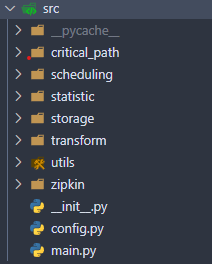
\includegraphics[width=0.35\textwidth]{resources/ch4/packages.png}
	\caption{Implementasi modul sebagai \textit{package}}
	\label{package}
\end{figure} 

%Gambar \ref{api_docs} adalah hasil tangkapan layar dokumentasi API yang disediakan oleh FastAPI. 
%\begin{figure}[!htb]
%	\centering
%	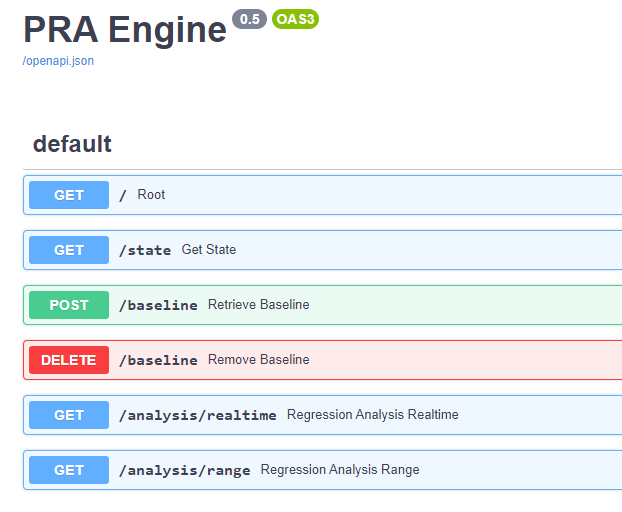
\includegraphics[width=0.5\textwidth]{resources/ch4/api_docs.png}
%	\caption{Dokumentasi API}
%	\label{api_docs}
%\end{figure} 
%
%Berikut adalah tangkapan layar dari hasil pemanggilan beberapa \textit{endpoint} yang dilakukan dengan aplikasi Postman \footnote{\url{https://www.postman.com/}}.
%\begin{figure}[h!]
%	\centering
%	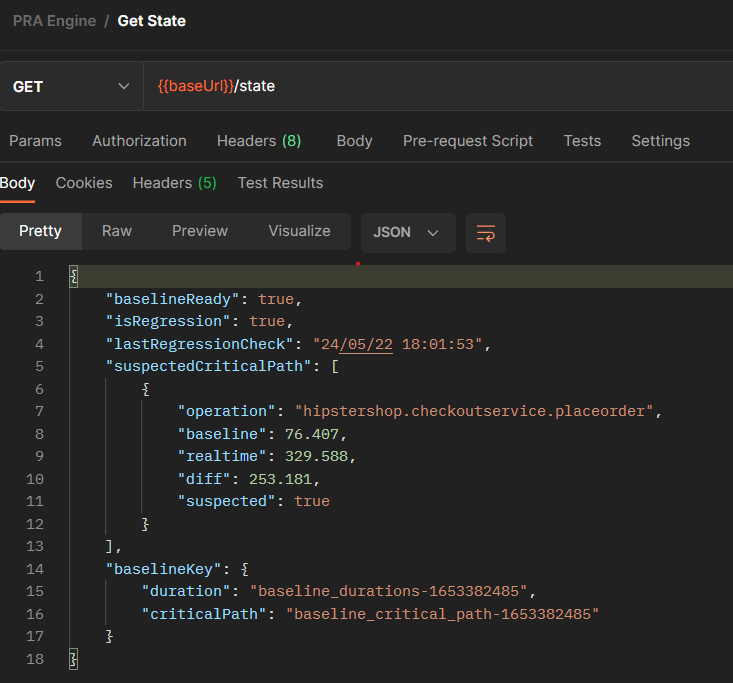
\includegraphics[width=0.75\textwidth]{resources/ch4/result_state.png}
%	\caption{Hasil pemanggilan \textit{endpoint} \texttt{/state}}
%	\label{api_state}
%\end{figure} 
%\begin{figure}[h!]
%	\centering
%	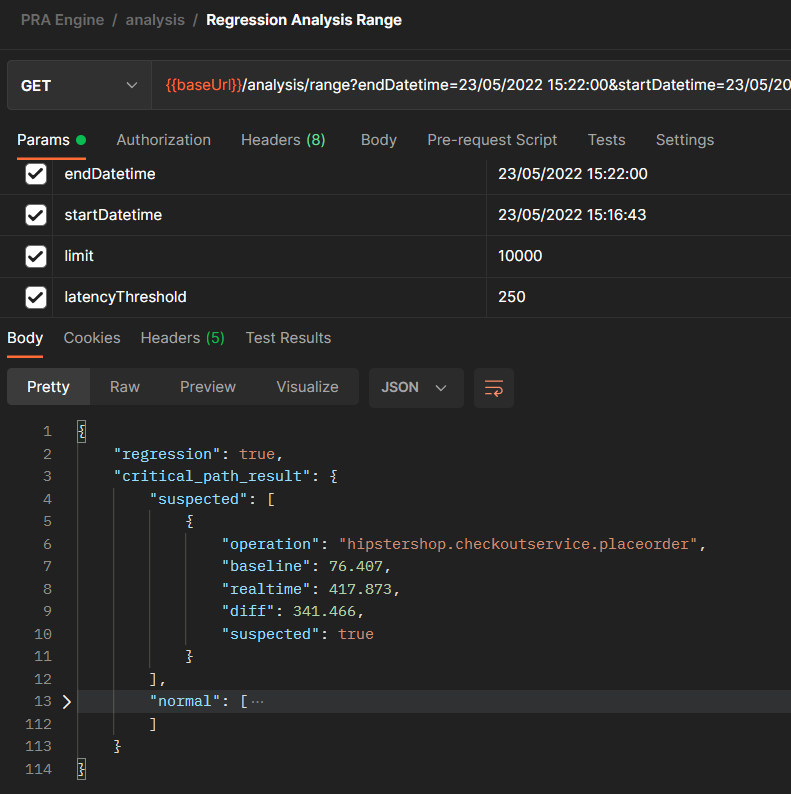
\includegraphics[width=0.75\textwidth]{resources/ch4/result_analysis_range.png}
%	\caption{Hasil pemanggilan \textit{endpoint} \texttt{/analysis/range}}
%	\label{api_analysis_range}
%\end{figure} 
%\begin{figure}[h!]
%	\centering
%	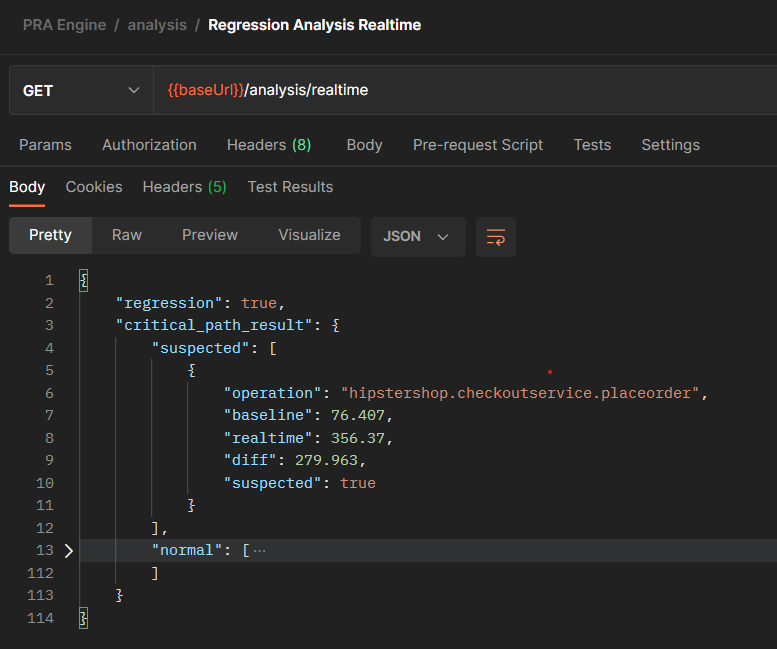
\includegraphics[width=0.75\textwidth]{resources/ch4/result_analysis_realtime.png}
%	\caption{Hasil pemanggilan \textit{endpoint} \texttt{/analysis/realtime}}
%	\label{api_analysis_realtime}
%\end{figure} 

\pagebreak


\subsubsection{Model dan Struktur Data}
Sistem PRA yang dibuat bergantung pada data \textit{trace} yang diperoleh dari Zipkin. Data tersebut tidak bisa begitu saja digunakan untuk menjalankan fungsi-fungsi dari \textit{engine} PRA sesuai yang terdapat pada gambar \ref{alur-pra} dan perlu ditransformasikan menjadi model dan struktur data yang lebih bermakna seperti yang telah disebutkan pada EM-2 di tabel \ref{engine-module}.

Dalam dokumentasinya, Zipkin menyediakan keterangan mengenai model data \textit{trace} yang digunakannya seperti yang terdapat pada \citep{zipkin-data}. Model data yang digunakan Zipkin terbagi menjadi dua yaitu \textit{span} dan \textit{trace}. \textit{Trace} sendiri merupakan serangkaian \textit{span} dengan id \textit{trace} sama yang merepresentasikan alur jalannya sebuah \textit{request} dalam sebuah \textit{service} yang telah terinstrumentasi, sementara \textit{span} merepresentasikan salah satu operasi yang terjadi sepanjang sebuah \textit{request}. Beberapa informasi yang terdapat pada data \textit{span} antara lain adalah informasi mengenai \textit{trace} dimana \textit{span} itu berada, metadata mengenai operasi yang direpresentasikan \textit{span}, durasi atau \textit{latency} dari operasi.

Sementara itu, untuk memenuhi fungsi-fungsi pada sistem PRA, data yang bersumber dari Zipkin perlu ditransformasikan menjadi struktur data yang sesuai dengan kebutuhan masing-masing tahap analisis. Dari rancangan alur sistem PRA, terdapat tiga tahap analisis yang akan dilakukan, yaitu tahap pendeteksian regresi dengan analisis statistik Kolmogorov-Smirnov, tahap analisis korelasi, dan tahap analisis \textit{critical path}.

Pada tahap pendeteksian regresi dengan tes statistik Kolmogorov-Smirnov (K-S), data yang diperlukan adalah data \textit{latency} atau durasi operasi dari \textit{span} yang dimiliki oleh Zipkin. Tes K-S akan membandingkan dua buah sampel data \textit{latency} dan akan menghasilkan hipotesis apakah kedua fungsi tersebut berada pada distribusi yang sama.

Pada tahap analisis \textit{critical path}, data yang dibutuhkan adalah pasangan \textit{key-value} dari nama operasi yang terrekam oleh Zipkin dan juga nilai \textit{latency} dari operasi tersebut. Data \textit{critical path} akan disimpan sebagai struktur data \textit{map} yang sesuai untuk menyimpan data berbentuk pasangan \textit{key-value}. Data ini akan didapatkan dari data \textit{trace} bawaan Zipkin yang sudah memiliki informasi mengenai \textit{critical path} dan juga nilai \textit{latency} nya masing-masing. 

\subsubsection{Algoritme}
Setelah pada subbab sebelumnya didefinisikan struktur data yang akan digunakan untuk merepresentasikan beberapa model seperti yang ada pada gambar \ref{alur-pra}, pada subbab ini akan didefinisikan algoritme penting yang akan digunakan untuk melakukan pendeteksian regresi pada aplikasi Microservice. 

Algoritme yang didasarkan pada tes statistik Kolmogorov-Smirnov ini akan membandingkan dua buah sampel data dan akan menentukan apakah kedua sampel tersebut berasal dari distribusi yang sama. Pertama-tama kita definisikan dua hipotesis yaitu $h_{0}$ atau hipotesis \textit{null} yang menyatakan bahwa kedua sampel data berasal dari distribusi yang sama dan $h_{a}$ atau hipotesis alternatif yang menyatakan bahwa kedua sampel data berasal dari dua distribusi yang berbeda. 

Kemudian akan dijalankan tes statistik K-S yang dilakukan menggunakan fungsi dari \textit{library}
SciPy yang akan menghasilkan dua buah nilai, yaitu \texttt{statistic} dan \texttt{p-value}. Jika nilai \texttt{p-value} lebih kecil dari nilai signifikan, atau \texttt{alpha} pada fungsi,  maka kita dapat menolak $h_{0}$ dan menerima $h_{a}$. Jika  \texttt{p-value} tidak lebih kecil dari nilai signifikan, maka selanjutnya adalah membandingkan antara nilai \texttt{statistic} dan \texttt{critical value}. \texttt{Critical value} sendiri merupakan sebuah titik pada tes hipotesis yang akan dibandingkan pada hasil nilai \texttt{statistic} yang akan digunakan untuk menolak atau menerima hipotesis \textit{null}. Jika nilai \texttt{statistic} lebih besar dari nilai \texttt{critical value}, maka kita dapat menolak $h_{0}$ dan menerima $h_{a}$ atau artinya kedua sampel data berasal dari distribusi yang berbeda. Namun jika  nilai \texttt{statistic} lebih kecil dari nilai \texttt{critical value}, kita tidak dapat menolak $h_{0}$ atau artinya kedua sampel data berasal dari distribusi yang sama.


Jika kedua sampel ternyata berasal dari distribusi yang berbeda, maka dapat dicurigai telah terjadi regresi pada aplikasi sebab distribusi dari data yang bersumber dari  \textit{trace} \textit{real-time} berbeda dengan distribusi dari data \textit{trace} \textit{baseline} yang dijadikan acuan kinerja normal aplikasi.

\lstinputlisting[captionpos=b, language=Python,caption={Algoritme tes statistik Kolmogorov-Smirnov}]{codes/ch4/ks.py}


\subsection{\textit{User Interface}}
Komponen lainnya yang akan diimplementasikan pada Tugas Akhir ini adalah komponen \textit{User Interface} (UI). Komponen ini akan menjadi antarmuka yang dapat digunakan untuk mengetahui \textit{state} dari sistem PRA. Fungsionalitas yang akan dibuat pada komponen UI akan dijabarkan pada tabel kebutuhan  fungsional \ref{ui-functional}.
\begin{small}
	\begin{longtable}{ | p{3cm} | p{9cm} | }
		\caption{Tabel kebutuhan fungsional komponen UI}
		\label{ui-functional}                                                           
		\\ \hline
		\centering\bfseries{ID} & \centering\bfseries{Deskripsi} \tabularnewline \hline
		\endfirsthead
		\centering{UI-1} & UI dapat menampilkan status pendeteksian regresi  \\ \hline
		\centering{UI-2} & UI dapat menampilkan hasil analisis \textit{critical path} berupa nama operasi dan nilai \textit{latency} \\ \hline

	\end{longtable}
\end{small}

\subsubsection{Hasil implementasi}
Berikut adalah tangkapan layar hasil implementasi komponen \textit{User Interface}.

\begin{figure}[!htb]
	\centering
	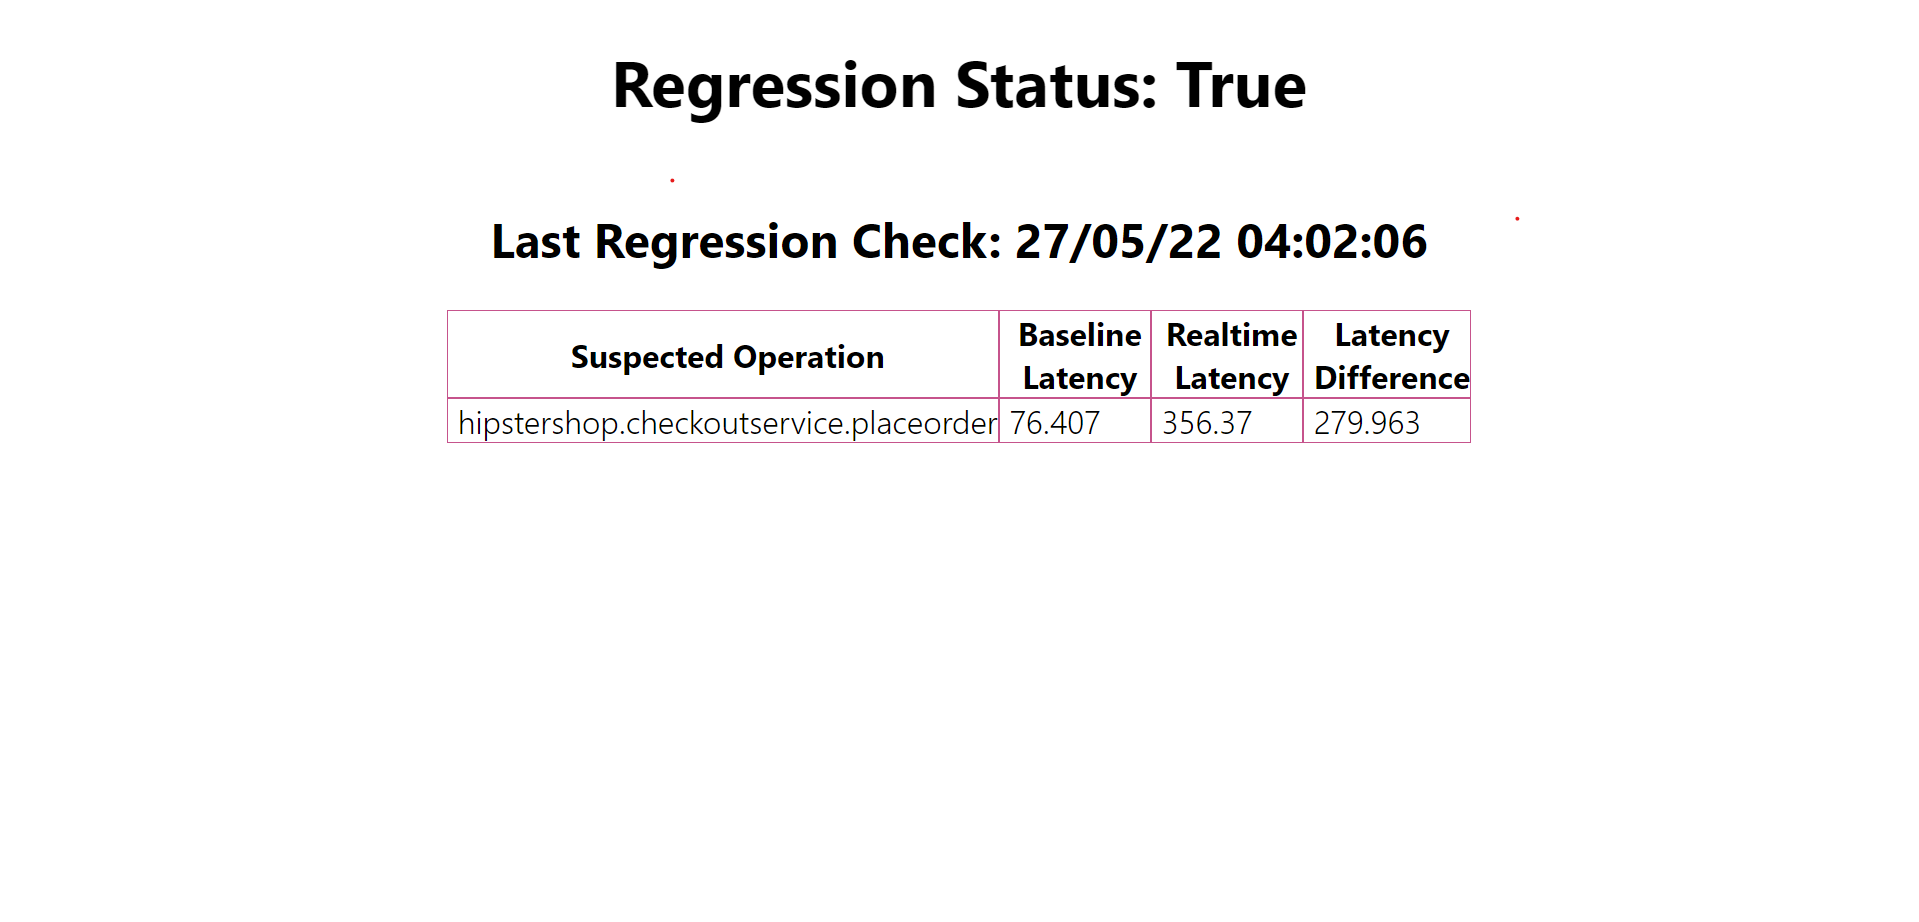
\includegraphics[width=1\textwidth]{resources/ch4/ui.png}
	\caption{Tangkapan layar UI}
	\label{ui}
\end{figure}

\section{Pengujian}
Untuk mengetahui keberhasilan dari sistem yang telah diimplementasikan, akan dilakukan pengujian sebagai berikut.
\subsection{Tujuan Pengujian}
Pengujian sistem PRA akan dilakukan dengan tujuan untuk:
\begin{enumerate}
	\item Mengukur keberhasilan sistem PRA dalam mendeteksi regresi
	\item Mengukur keberhasilan sistem PRA dalam menentukan kandidat sumber regresi
	\item Mengukur \textit{overhead} yang diakibatkan oleh sistem PRA dengan
	indikator berupa penggunaan memori dan pemanfaatan CPU.
\end{enumerate}

Tujuan utama pengujian sistem \textit{Performance Regression Analysis} adalah untuk menguji apakah sistem dapat mendeteksi terjadinya regresi atau penurunan kinerja dengan indikasi peningkatan nilai \textit{latency} yang disebabkan oleh perubahan yang terjadi pada aplikasi. Perubahan tersebut dapat berupa penambahan atau \textit{update} fitur, hasil perbaikan \textit{bug}, dsb. Sehingga kasus-kasus yang akan diujikan utamanya merupakan simulasi terjadinya perubahan pada level aplikasi \textit{microservice}. Namun sebagai perbandingan akan terdapat juga kasus-kasus yang menyimulasikan perubahan yang terjadi di luar level aplikasi seperti peningkatan jumlah pengguna dan peningkatan \textit{load} pada Load Generator pada \textit{service}-\textit{service} tertentu. Kasus pengujian akan dijelaskan lebih lanjut pada subbab \ref{metode-pengujian}.

\subsection{Lingkungan Pengujian}
Pengujian akan dilakukan pada Google Kubernetes Engine dengan spesifikasi yang dipaparkan pada tabel \ref{testing-env}.
\begin{small}
	\begin{longtable}{ | p{5cm} | p{8cm} | }
		\caption{Spesifikasi Lingkungan Pengujian}
		\label{testing-env}                                                           
		\\ \hline
		\centering\bfseries{Layanan Kubernetes} & \centering\bfseries{Google Kubernetes Engine} \tabularnewline \hline
		\endfirsthead
		\textit{Operating System} & Container Optimized OS (COS) \\ \hline
		\textit{Instance Type} & n1-standard-2 (2 vCPU,  7,5 GiB RAM) \\ \hline
		Jumlah Node & 3 \\ \hline
		
	\end{longtable}
\end{small}

\subsection{Aplikasi Pengujian}
Aplikasi yang akan digunakan untuk melakukan pengujian sistem PRA adalah aplikasi Hipster Shop yang merupakan aplikasi \textit{e-commerce} berbasis web yang dibuat untuk mendemostrasikan berbagai macam teknologi yang dimiliki oleh Google. Seperti pada gambar \ref{butiq-arch}, Hipster Shop terdiri atas 10 microservice yang saling berkomunikasi melalui gRPC. Selain itu Hipster Shop juga memiliki load generator yang secara terus menerus mengirimkan request untuk menyimulasikan alur belanja pengguna. Hipster Shop sudah memiliki load generator yang dibuat menggunakan Locust
untuk menyimulasikan pengunaan aplikasi oleh sejumlah user. Aplikasi Hipster Shop akan dimodifikasi dengan diinstumentasikan menggunakan Zipkin untuk menyimulasikan lingkungan \textit{distributed tracing} yang menggunakan Zipkin.
\begin{figure}[!htb]
	\centering
	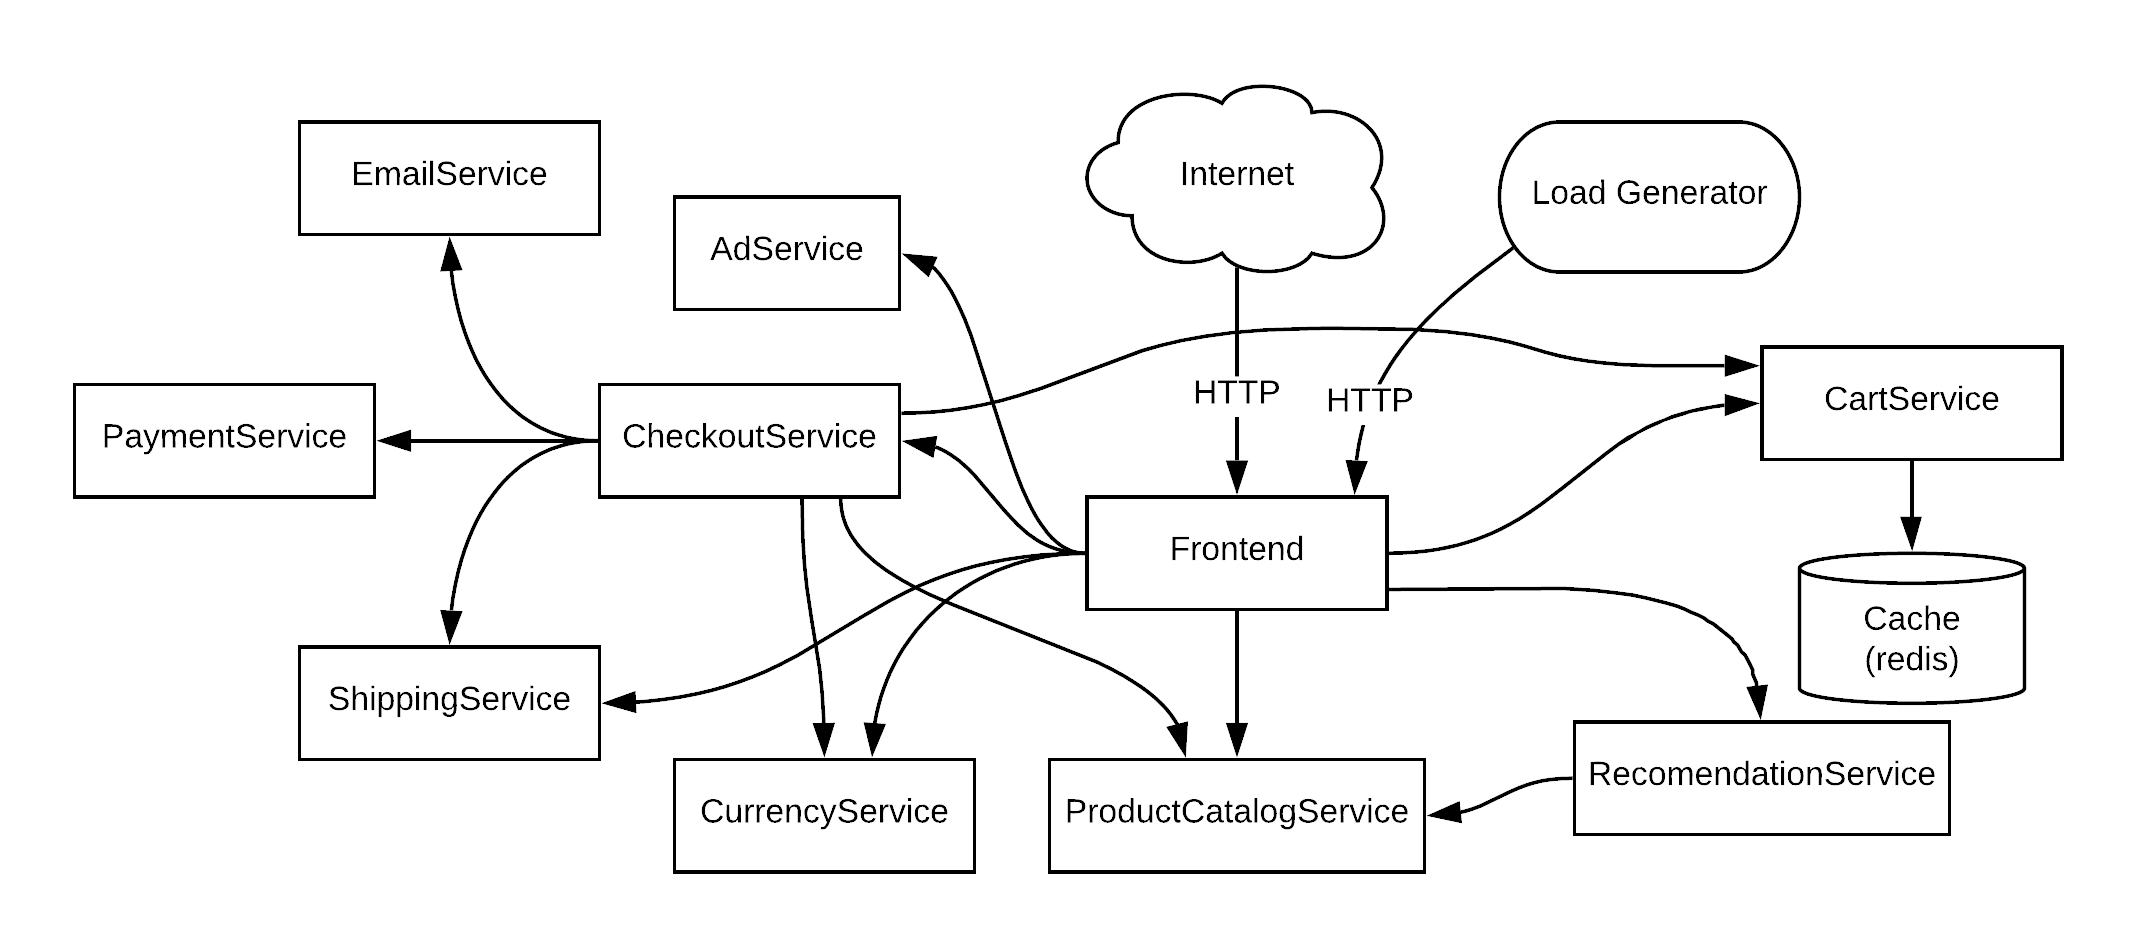
\includegraphics[width=1\textwidth]{resources/ch4/hipster-arch.png}
	\caption{Arsitektur aplikasi Hipster Shop}
	\label{butiq-arch}
\end{figure}


\subsection{Metode Pengujian}
\label{metode-pengujian}
Untuk melakukan pengujian pada sistem PRA yang telah dibuat, \textit{service} yang ada pada Hipster Shop akan dimodifikasi untuk meniru perilaku dari \textit{service} yang mengalami regresi kinerja. Ada dua metode utama yang dapat dilakukan untuk membuat perilaku regresi pada \textit{service} yaitu dengan menambahkan perintah \textit{sleep} dan menambahkan \textit{loop} dengan operasi \textit{dereference} sebuah variabel yang membutuhkan banyak usaha dari CPU untuk menyelesaikannya sehingga diharapkan fungsi-fungsi tersebut akan memiliki \textit{latency} yang lebih besar. 

Ada dua tahap yang akan dilakukan untuk melakukan pengujian ini, pertama tahap pengambilan data \textit{baseline}. Data \textit{baseline} akan diambil dengan menyimulasikan pengunaan aplikasi dengan menggunakan Load Generator yang akan dijalankan dengan variabel \textbf{25 User} dan \textbf{5 Spawn Rate} selama \textbf{1 jam}. Data \textit{baseline} ini kemudian akan disimpan oleh \textit{engine} untuk dipergunakan di kasus-kasus pengujian selanjutnya. Tahap selanjutnya adalah melakukan pengujian dengan kasus-kasus yang akan dijelaskan lebih lanjut.

Terdapat dua jenis kasus uji yang akan diujikan pada sistem. Jenis pertama adalah kasus-kasus yang menyimulasikan regresi dengan melakukan perubahan yang terjadi di level aplikasi dengan cara melakukan modifikasi secara sengaja di level kode. Kasus pertama akan memiliki ID dengan awalan \textbf{SI} menandakan \textit{skenario-internal}. Jenis kedua adalah kasus-kasus yang menyimulasikan regresi dengan meningkatkan jumlah pengguna dan \textit{load} pada Load Generator. Kasus kedua akan memliki ID dengan awalan \textbf{SE} menandakan \textit{skenario-eksternal}. Tabel \ref{testcase} akan menjelaskan kasus-kasus pengujian sistem.

Pengujian pada tabel \ref{testcase} seluruhnya dilakukan dengan cara terlebih dahulu melakukan \textit{deployment} masing-masing kasus uji di lingkungan Kubernetes kemudian menjalankan aplikasi Load Generator sesuai dengan spesifikasi masing-masing kasus uji selama $\pm 5$ menit. Hasil akhir dari setiap kasus uji akan berupa \textit{response} dalam bentuk JSON dari API dan juga \textit{log} dari aplikasi untuk mengetahui hasil tes  statistik K-S yang akan dipergunakan untuk keperluan analisis selanjutnya.
\begin{table}[htb]
	\caption{Tabel kasus uji}
	
	\begin{adjustwidth}{-1.5cm}{}
		% Please add the following required packages to your document preamble:
		% \usepackage{multirow}
		% \usepackage[table,xcdraw]{xcolor}
		% If you use beamer only pass "xcolor=table" option, i.e. \documentclass[xcolor=table]{beamer}
		\begin{tabular}{llccl}
			\hline
			\rowcolor[HTML]{009901} 
			\multicolumn{1}{c}{\cellcolor[HTML]{009901}{\color[HTML]{FFFFFF} \textbf{ID}}} &
			\multicolumn{1}{c}{\cellcolor[HTML]{009901}{\color[HTML]{FFFFFF} \textbf{Service (Fungsi)}}} &
			\multicolumn{1}{l}{\cellcolor[HTML]{009901}{\color[HTML]{FFFFFF} \textbf{Extra Latency}}} &
			\multicolumn{1}{l}{\cellcolor[HTML]{009901}{\color[HTML]{FFFFFF} \textbf{User}}} &
			{\color[HTML]{FFFFFF} \textbf{Keterangan}} \\ \hline
			\multicolumn{1}{|l|}{\textbf{SI1}} &
			\multicolumn{1}{l|}{CheckoutService (placeorder)} &
			\multicolumn{1}{c|}{100ms} &
			\multicolumn{1}{c|}{25} &
			\multicolumn{1}{l|}{Kasus extra latency \#1} \\ \hline
			\multicolumn{1}{|l|}{\textbf{SI2}} &
			\multicolumn{1}{l|}{CheckoutService (placeorder)} &
			\multicolumn{1}{c|}{250ms} &
			\multicolumn{1}{c|}{25} &
			\multicolumn{1}{l|}{Kasus extra latency \#2} \\ \hline
			\multicolumn{1}{|l|}{\textbf{SI3}} &
			\multicolumn{1}{l|}{CheckoutService (placeorder)} &
			\multicolumn{1}{c|}{350ms} &
			\multicolumn{1}{c|}{25} &
			\multicolumn{1}{l|}{Kasus extra latency \#3} \\ \hline
			\multicolumn{1}{|l|}{\textbf{SI4}} &
			\multicolumn{1}{l|}{CheckoutService (placeorder)} &
			\multicolumn{1}{c|}{250ms} &
			\multicolumn{1}{c|}{75} &
			\multicolumn{1}{l|}{\begin{tabular}[c]{@{}l@{}}Kasus extra latency \\ dengan peningkatan user \#1\end{tabular}} \\ \hline
			\multicolumn{1}{|l|}{\textbf{SI5}} &
			\multicolumn{1}{l|}{CheckoutService (placeorder)} &
			\multicolumn{1}{c|}{250ms} &
			\multicolumn{1}{c|}{150} &
			\multicolumn{1}{l|}{\begin{tabular}[c]{@{}l@{}}Kasus extra latency \\ dengan peningkatan user \#1\end{tabular}} \\ \hline
			\multicolumn{1}{|l|}{\textbf{SI6}} &
			\multicolumn{1}{l|}{CheckoutService (placeorder)} &
			\multicolumn{1}{c|}{-} &
			\multicolumn{1}{c|}{25} &
			\multicolumn{1}{l|}{Kasus peningkatan kerja CPU} \\ \hline
			\multicolumn{1}{|l|}{} &
			\multicolumn{1}{l|}{CheckoutService (placeorder)} &
			\multicolumn{1}{c|}{} &
			\multicolumn{1}{c|}{} &
			\multicolumn{1}{l|}{} \\ \cline{2-2}
			\multicolumn{1}{|l|}{} &
			\multicolumn{1}{l|}{\begin{tabular}[c]{@{}l@{}}ProductCatalog (getproduct,\\ listproducts)\end{tabular}} &
			\multicolumn{1}{c|}{} &
			\multicolumn{1}{c|}{} &
			\multicolumn{1}{l|}{} \\ \cline{2-2}
			\multicolumn{1}{|l|}{} &
			\multicolumn{1}{l|}{ShippingService (getquote)} &
			\multicolumn{1}{c|}{} &
			\multicolumn{1}{c|}{} &
			\multicolumn{1}{l|}{} \\ \cline{2-2}
			\multicolumn{1}{|l|}{\multirow{-4}{*}{\textbf{SI7}}} &
			\multicolumn{1}{l|}{\begin{tabular}[c]{@{}l@{}}RecommendationService \\ (listrecommendations)\end{tabular}} &
			\multicolumn{1}{c|}{\multirow{-4}{*}{250ms}} &
			\multicolumn{1}{c|}{\multirow{-4}{*}{25}} &
			\multicolumn{1}{l|}{\multirow{-4}{*}{\begin{tabular}[c]{@{}l@{}}Kasus extra latency\\  dengan beberapa service\end{tabular}}} \\ \hline
			\multicolumn{1}{|l|}{\textbf{SE1}} &
			\multicolumn{1}{l|}{All Normal} &
			\multicolumn{1}{c|}{-} &
			\multicolumn{1}{c|}{75} &
			\multicolumn{1}{l|}{\begin{tabular}[c]{@{}l@{}}Tidak ada peningkatan latency\\ dengan peningkatan pengguna \#1\end{tabular}} \\ \hline
			\multicolumn{1}{|l|}{\textbf{SE2}} &
			\multicolumn{1}{l|}{All Normal} &
			\multicolumn{1}{c|}{-} &
			\multicolumn{1}{c|}{150} &
			\multicolumn{1}{l|}{\begin{tabular}[c]{@{}l@{}}Tidak ada peningkatan latency\\ dengan peningkatan pengguna \#1\end{tabular}} \\ \hline
			\multicolumn{1}{|l|}{\textbf{SE3}} &
			\multicolumn{1}{l|}{\begin{tabular}[c]{@{}l@{}}Checkout load \\ increased to 100 in loadgen\end{tabular}} &
			\multicolumn{1}{c|}{-} &
			\multicolumn{1}{c|}{25} &
			\multicolumn{1}{l|}{Tes pengujian load external \#1} \\ \hline
			\multicolumn{1}{|l|}{\textbf{SE4}} &
			\multicolumn{1}{l|}{\begin{tabular}[c]{@{}l@{}}Currency load\\  increased to 100 in loadgen\end{tabular}} &
			\multicolumn{1}{c|}{-} &
			\multicolumn{1}{c|}{25} &
			\multicolumn{1}{l|}{Tes pengujian load external \#2} \\ \hline
		\end{tabular}
	\end{adjustwidth}
	\label{testcase}
\end{table}


\subsection{Hasil Pengujian Regresi}
Berikut adalah hasil pengujian yang telah dilakukan pada sistem PRA sesuai dengan kasus uji \ref{testcase}.

\subsubsection{Kasus SI1}
Seperti yang terlihat pada gambar \ref{result_json_1}, regresi tidak terdeteksi pada kasus ini sehingga analisis \textit{critical path} tidak dijalankan.
\begin{figure}[!htb]
	\centering
	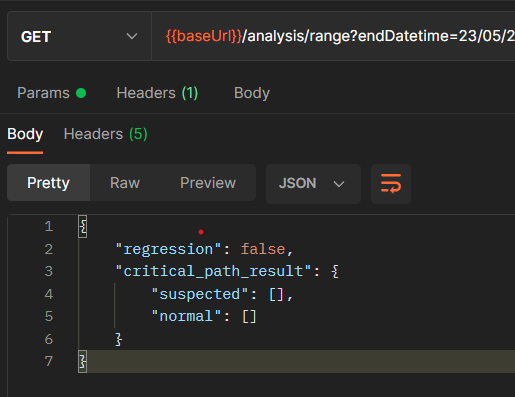
\includegraphics[width=0.75\textwidth]{resources/ch4/json/1.png}
	\caption{\textit{Response} JSON hasil pengujian kasus \textbf{SI1}}
	\label{result_json_1}
\end{figure}

\pagebreak

%\begin{figure}[!htb]
%	\centering
%	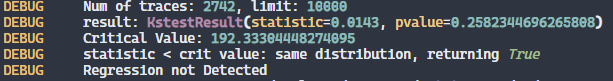
\includegraphics[width=1\textwidth]{resources/ch4/log/1-log.png}
%	\caption{\textit{Log} hasil pengujian kasus SI1}
%	\label{result_log_1}
%\end{figure}

\subsubsection{Kasus SI2}
Seperti yang terlihat pada gambar \ref{result_json_2}, regresi terdeteksi dan analisis \textit{critical path} dapat menentukan sumber regresi yaitu operasi \texttt{placeorder} dari \textit{service} \texttt{CheckoutService}.
\begin{figure}[!htb]
	\centering
	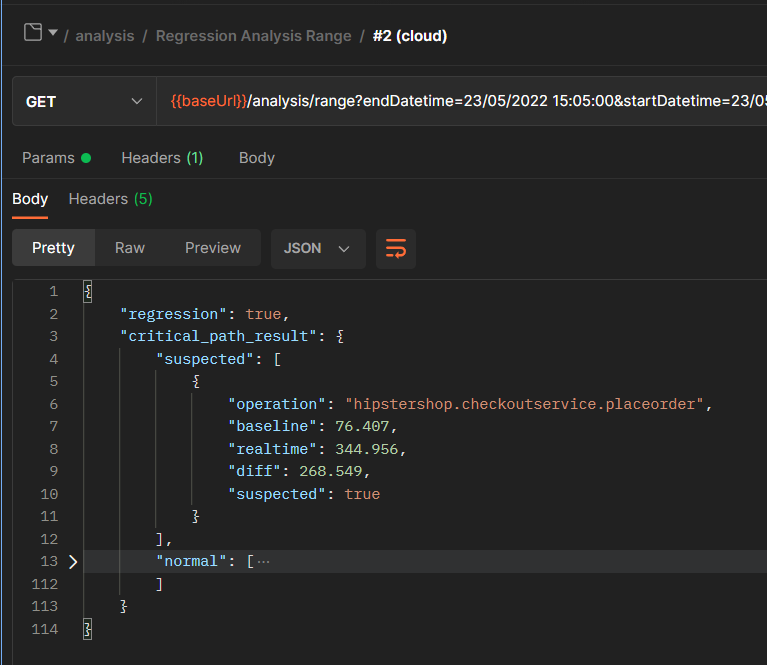
\includegraphics[width=0.75\textwidth]{resources/ch4/json/2.png}
	\caption{\textit{Response} JSON hasil pengujian kasus \textbf{SI2}}
	\label{result_json_2}
\end{figure}

%\begin{figure}[!htb]
%	\centering
%	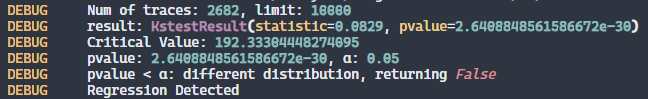
\includegraphics[width=1\textwidth]{resources/ch4/log/2-log.png}
%	\caption{\textit{Log} hasil pengujian kasus SI3}
%	\label{result_log_2}
%\end{figure}
\pagebreak

\subsubsection{Kasus SI3}
Seperti yang terlihat pada gambar \ref{result_json_3}, regresi terdeteksi dan analisis \textit{critical path} dapat menentukan sumber regresi yaitu operasi \texttt{placeorder} dari \textit{service} \texttt{CheckoutService}.
\begin{figure}[!htb]
	\centering
	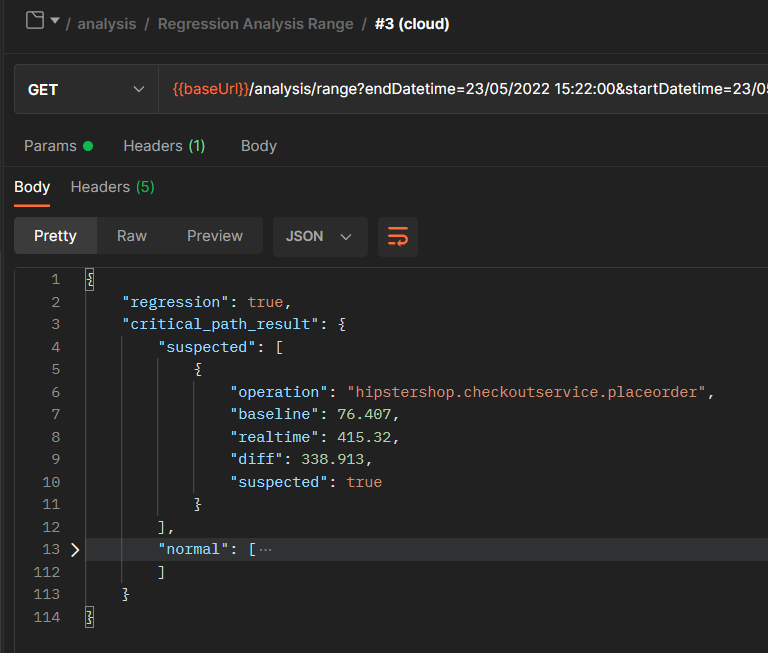
\includegraphics[width=0.75\textwidth]{resources/ch4/json/3.png}
	\caption{\textit{Response} JSON hasil pengujian kasus \textbf{SI3}}
	\label{result_json_3}
\end{figure}

%\begin{figure}[!htb]
%	\centering
%	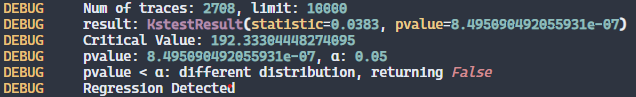
\includegraphics[width=1\textwidth]{resources/ch4/log/3-log.png}
%	\caption{\textit{Log} hasil pengujian kasus SI3}
%	\label{result_log_3}
%\end{figure}
%\pagebreak
\subsubsection{Kasus SI4}
Seperti yang terlihat pada gambar \ref{result_json_4}, regresi terdeteksi dan analisis \textit{critical path} dapat menentukan sumber regresi yaitu operasi \texttt{placeorder} dari \textit{service} \texttt{CheckoutService}.
\begin{figure}[!htb]
	\centering
	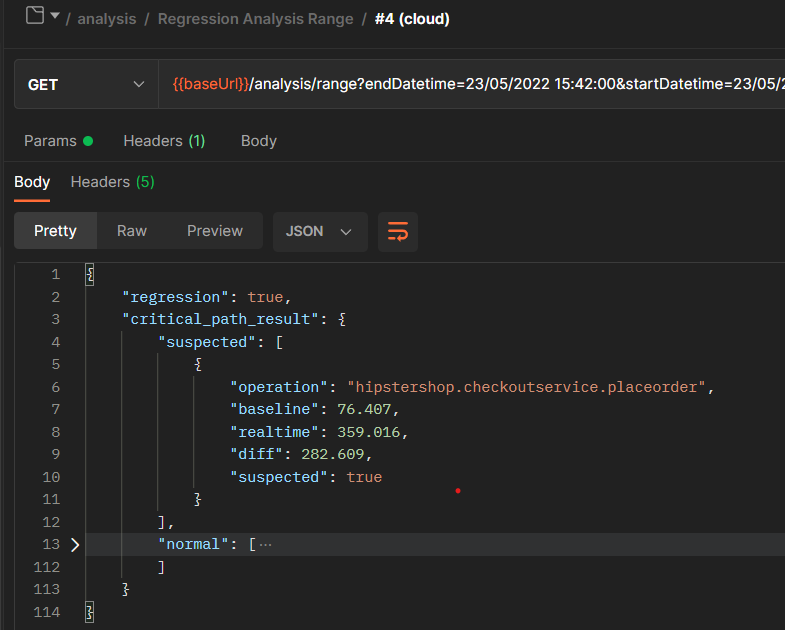
\includegraphics[width=0.75\textwidth]{resources/ch4/json/4.png}
	\caption{\textit{Response} JSON hasil pengujian kasus \textbf{SI4}}
	\label{result_json_4}
\end{figure}

%\begin{figure}[!htb]
%	\centering
%	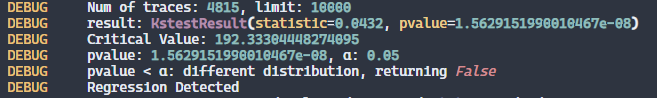
\includegraphics[width=1\textwidth]{resources/ch4/log/4-log.png}
%	\caption{\textit{Log} hasil pengujian kasus SI4}
%	\label{result_log_4}
%\end{figure}
\pagebreak

\subsubsection{Kasus SI5}
Seperti yang terlihat pada gambar \ref{result_json_5}, regresi terdeteksi dan analisis \textit{critical path} dapat menentukan sumber regresi yaitu operasi \texttt{placeorder} dari \textit{service} \texttt{CheckoutService}.
\begin{figure}[!htb]
	\centering
	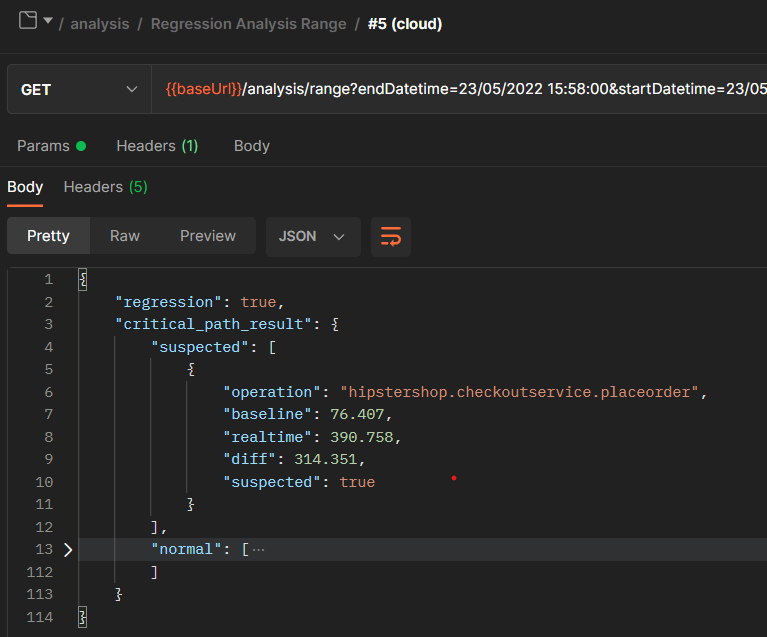
\includegraphics[width=0.75\textwidth]{resources/ch4/json/5.png}
	\caption{\textit{Response} JSON hasil pengujian kasus \textbf{SI5}}
	\label{result_json_5}
\end{figure}

%\begin{figure}[!htb]
%	\centering
%	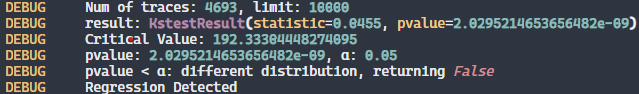
\includegraphics[width=1\textwidth]{resources/ch4/log/5-log.png}
%	\caption{\textit{Log} hasil pengujian kasus \textbf{SI5}}
%	\label{result_log_5}
%\end{figure}
\pagebreak

\subsubsection{Kasus SI6}
Seperti yang terlihat pada gambar \ref{result_json_6}, regresi terdeteksi dan analisis \textit{critical path} dapat menentukan sumber regresi yaitu operasi \texttt{placeorder} dari \textit{service} \texttt{CheckoutService}.
\begin{figure}[!htb]
	\centering
	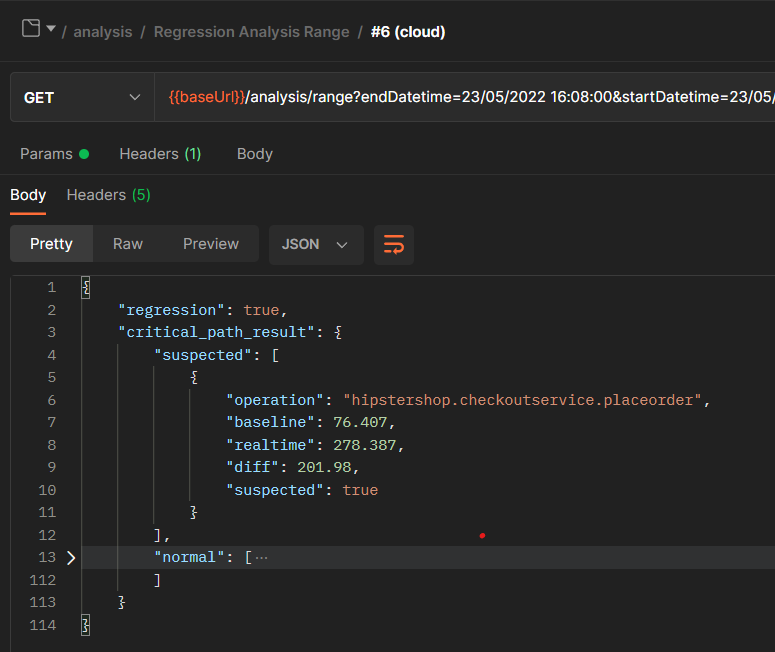
\includegraphics[width=0.75\textwidth]{resources/ch4/json/6.png}
	\caption{\textit{Response} JSON hasil pengujian kasus \textbf{SI6}}
	\label{result_json_6}
\end{figure}

%\begin{figure}[!htb]
%	\centering
%	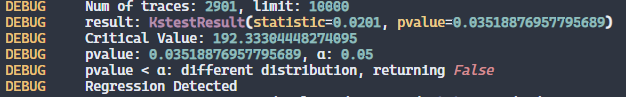
\includegraphics[width=1\textwidth]{resources/ch4/log/6-log.png}
%	\caption{\textit{Log} hasil pengujian kasus SI6}
%	\label{result_log_6}
%\end{figure}
%\pagebreak

\subsubsection{Kasus SI7}
Seperti yang terlihat pada gambar \ref{result_json_7}, regresi terdeteksi dan analisis \textit{critical path} dapat menentukan sumber regresi yaitu operasi \texttt{placeorder} dari \textit{service} \texttt{Checkout Service}, operasi \texttt{listrecommendations} dari \textit{service} \texttt{Recommendation Service}, operasi \texttt{getproduct} dari \textit{service} \texttt{ProductCatalog Service}, \texttt{listproducts} dari \textit{service} \texttt{ProductCatalog Service}, dan operasi \texttt{getquote} dari \textit{service} \texttt{Shipping Service}.

\begin{figure}[!htb]
	\centering
	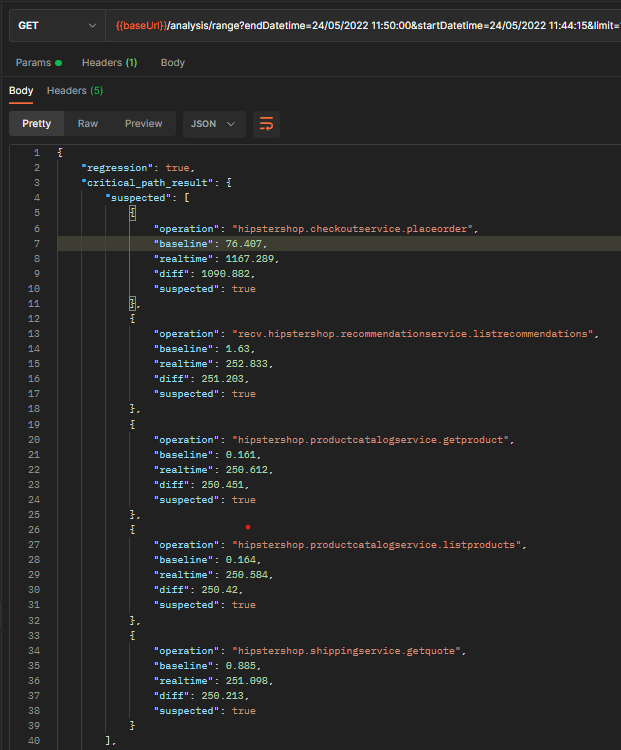
\includegraphics[width=0.75\textwidth]{resources/ch4/json/7.png}
	\caption{\textit{Response} JSON hasil pengujian kasus \textbf{SI7}}
	\label{result_json_7}
\end{figure}
%
%\begin{figure}[!htb]
%	\centering
%	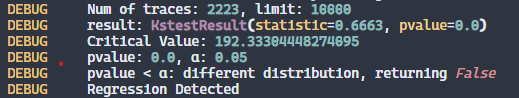
\includegraphics[width=1\textwidth]{resources/ch4/log/7-log.png}
%	\caption{\textit{Log} hasil pengujian kasus SI7}
%	\label{result_log_7}
%\end{figure}
\pagebreak

\subsubsection{Kasus SE1}
Seperti yang terlihat pada gambar \ref{result_json_6}, regresi terdeteksi namun analisis \textit{critical path} tidak dapat menentukan sumber regresi sebab selisih \textit{latency} tidak cukup besar sehingga tidak terdeteksi di data \textit{suspected}.
\begin{figure}[!htb]
	\centering
	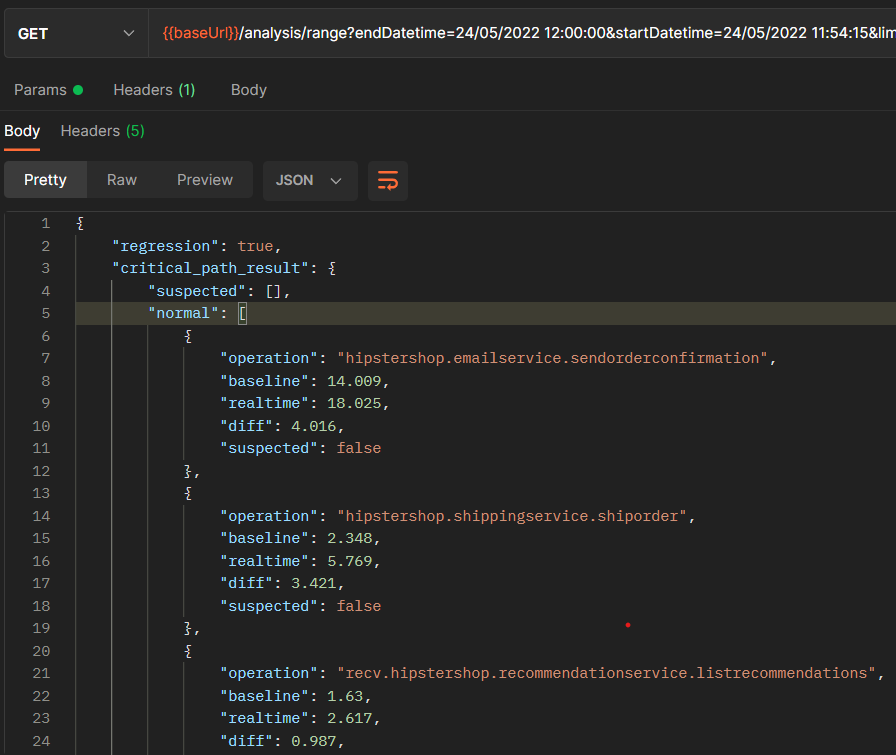
\includegraphics[width=0.75\textwidth]{resources/ch4/json/8.png}
	\caption{\textit{Response} JSON hasil pengujian kasus \textbf{SE1}}
	\label{result_json_8}
\end{figure}

%\begin{figure}[!htb]
%	\centering
%	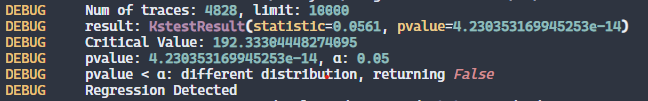
\includegraphics[width=1\textwidth]{resources/ch4/log/8-log.png}
%	\caption{\textit{Log} hasil pengujian kasus SE1}
%	\label{result_log_8}
%\end{figure}
\pagebreak

\subsubsection{Kasus SE2}
Seperti yang terlihat pada gambar \ref{result_json_6}, regresi terdeteksi namun analisis \textit{critical path} tidak dapat menentukan sumber regresi sebab selisih \textit{latency} tidak cukup besar sehingga tidak terdeteksi di data \textit{suspected}.
\begin{figure}[!htb]
	\centering
	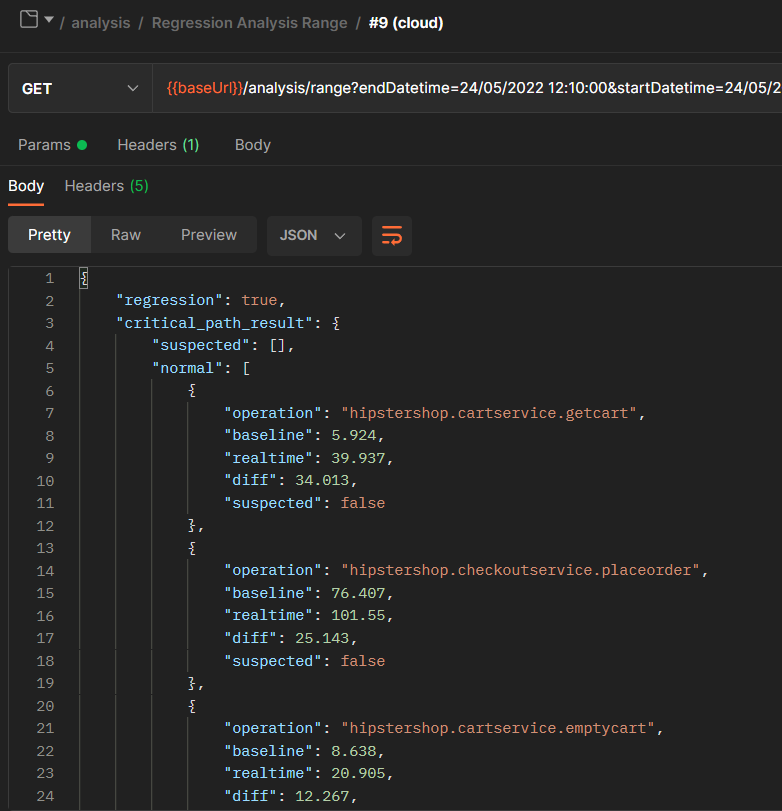
\includegraphics[width=0.75\textwidth]{resources/ch4/json/9.png}
	\caption{\textit{Response} JSON hasil pengujian kasus \textbf{SE2}}
	\label{result_json_9}
\end{figure}

%\begin{figure}[!htb]
%	\centering
%	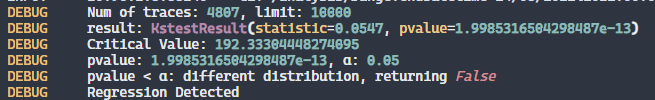
\includegraphics[width=1\textwidth]{resources/ch4/log/9-log.png}
%	\caption{\textit{Log} hasil pengujian kasus SE2}
%	\label{result_log_9}
%\end{figure}
\pagebreak

\subsubsection{Kasus SE3}
Seperti yang terlihat pada gambar \ref{result_json_6}, regresi terdeteksi namun analisis \textit{critical path} tidak dapat menentukan sumber regresi sebab selisih \textit{latency} tidak cukup besar sehingga tidak terdeteksi di data \textit{suspected}.
\begin{figure}[!htb]
	\centering
	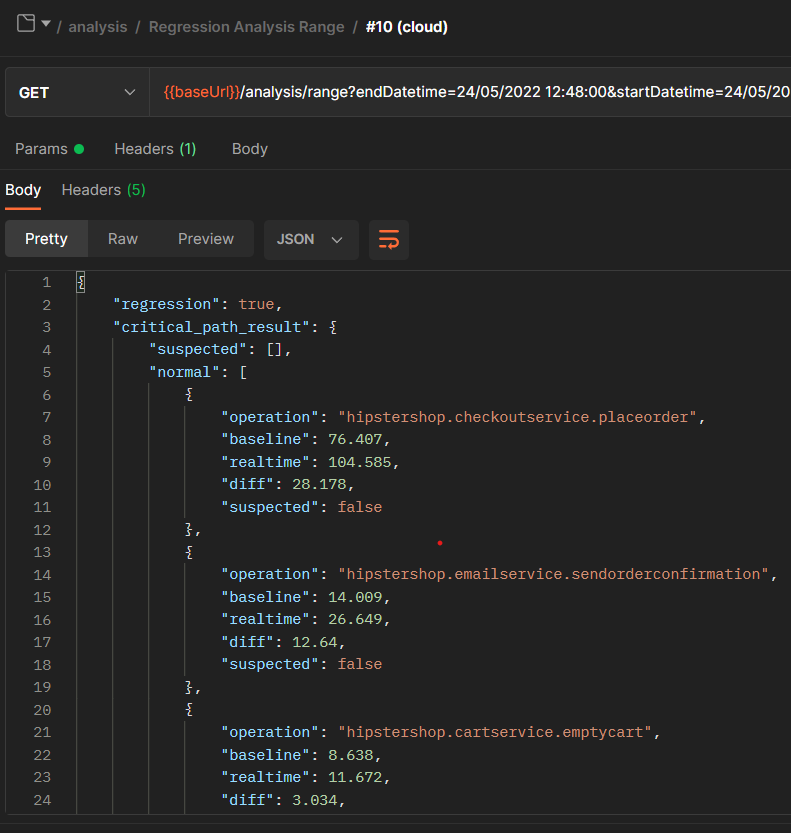
\includegraphics[width=0.75\textwidth]{resources/ch4/json/10.png}
	\caption{\textit{Response} JSON hasil pengujian kasus \textbf{SE3}}
	\label{result_json_10}
\end{figure}
%\begin{figure}[!htb]
%	\centering
%	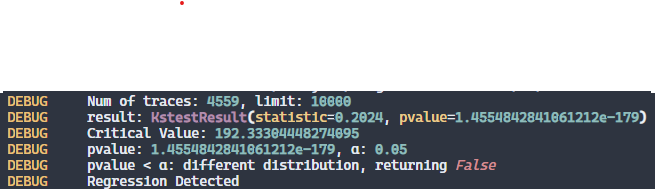
\includegraphics[width=1\textwidth]{resources/ch4/log/10-log.png}
%	\caption{\textit{Log} hasil pengujian kasus SE3}
%	\label{result_log_10}
%\end{figure}
\pagebreak

\subsubsection{Kasus SE4}
Seperti yang terlihat pada gambar \ref{result_json_6}, regresi terdeteksi namun analisis \textit{critical path} tidak dapat menentukan sumber regresi sebab selisih \textit{latency} tidak cukup besar sehingga tidak terdeteksi di data \textit{suspected}.
\begin{figure}[!htb]
	\centering
	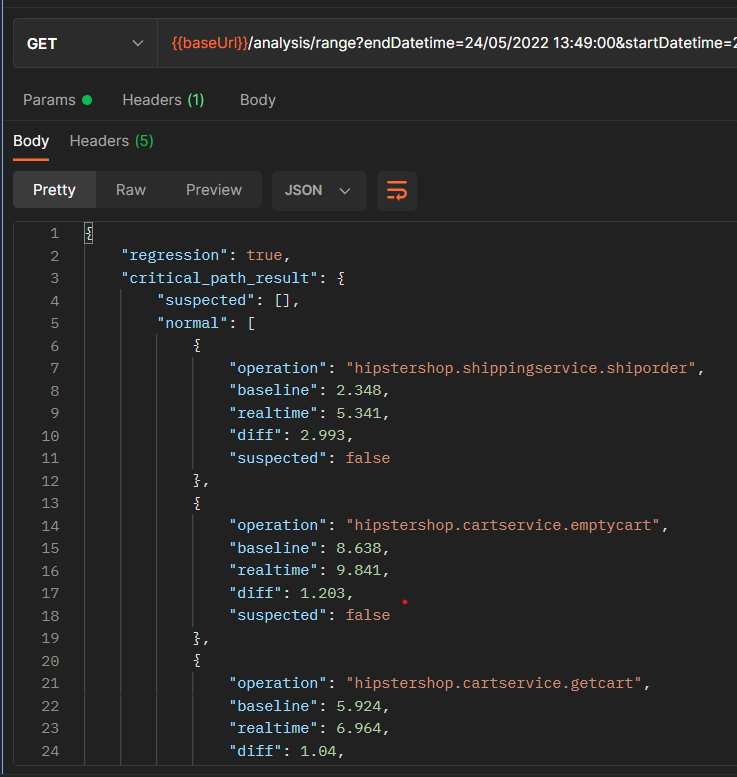
\includegraphics[width=0.75\textwidth]{resources/ch4/json/11.png}
	\caption{\textit{Response} JSON hasil pengujian kasus \textbf{SE4}}
	\label{result_json_9}
\end{figure}

%\begin{figure}[!htb]
%	\centering
%	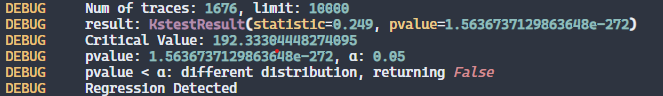
\includegraphics[width=1\textwidth]{resources/ch4/log/11-log.png}
%	\caption{\textit{Log} hasil pengujian kasus SE4}
%	\label{result_log_11}
%\end{figure}
\pagebreak

\subsubsection{Ringkasan hasil pengujian}
Tabel \ref{test-summary} mendeskripsikan ringkasan hasil pengujian yang telah dilakukan. Ada dua jenis metrik yang diukur pada setiap kasus yaitu keberhasilan pendeteksian regresi dan keberhasilan analisis \textit{critical path} dalam menentukan kandidat sumber terjadinya regresi. Pada kasus SI1, karena regresi tidak terdeteksi, analisis \textit{critical path} tidak dijalankan sehingga walaupun ada sebuah operasi yang memiliki \textit{latency} ekstra, PRA Engine tidak dapat mendeteksinya. Sementara untuk kasus SE1-SE4, PRA Engine dapat mendeteksi terjadinya regresi, namun hasil analisis \textit{critical path} tidak menghasilkan kandidat penyebab regresi sebab dari selisih \textit{latency} antara kasus regresi dan \textit{baseline} tidak lebih dari threshold \textit{default} yaitu 250ms.
\begin{table}[htb]
	\caption{Ringkasan hasil pengujian}
	\centering
	\begin{tabular}{|l|c|c|}
		\hline
		\rowcolor[HTML]{3166FF} 
		{\color[HTML]{FFFFFF} ID} &
		\multicolumn{1}{l|}{\cellcolor[HTML]{3166FF}{\color[HTML]{FFFFFF} Regresi terdeteksi}} &
		\multicolumn{1}{l|}{\cellcolor[HTML]{3166FF}{\color[HTML]{FFFFFF} Hasil Critical Path sesuai}} \\ \hline
		\textbf{SI1} & Tidak & Tidak \\ \hline
		\textbf{SI2} & Ya    & Ya    \\ \hline
		\textbf{SI3} & Ya    & Ya    \\ \hline
		\textbf{SI4} & Ya    & Ya    \\ \hline
		\textbf{SI5} & Ya    & Ya    \\ \hline
		\textbf{SI6} & Ya    & Ya    \\ \hline
		\textbf{SI7} & Ya    & Ya    \\ \hline
		\textbf{SE1} & Ya    & Tidak \\ \hline
		\textbf{SE2} & Ya    & Tidak \\ \hline
		\textbf{SE3} & Ya    & Tidak \\ \hline
		\textbf{SE4} & Ya    & Tidak \\ \hline
	\end{tabular}
	\label{test-summary}
\end{table}

\pagebreak

\subsection{Hasil Pengujian Kinerja}
Pada subbab ini akan disajikan hasil penggunaan CPU dan Memory pada masing-masing kasus uji beserta dengan rata-rata dan persentase keseluruhan \textit{resource} yang terdapat di Kubernetes. 
                           
\subsubsection{Kasus SI1}
Dari gambar \ref{result_cpu_1} dan \ref{result_mem_1} terlihat bahwa PRA Engine menggunakan \textit{resource} CPU sebanyak 0,042 vCPU dan Memory sebanyak 137,82 MiB. 

\begin{figure}[!htb]
	\centering
	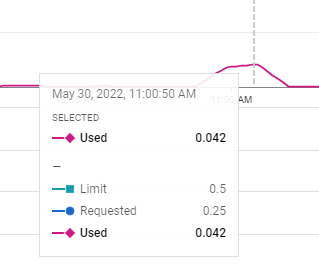
\includegraphics[width=0.5\textwidth]{resources/ch4/resource/1-cpu.png}
	\caption{Penggunaan CPU pada kasus \textbf{SI1}}
	\label{result_cpu_1}
\end{figure}

\begin{figure}[!htb]
	\centering
	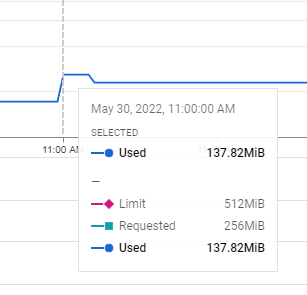
\includegraphics[width=0.5\textwidth]{resources/ch4/resource/1-mem.png}
	\caption{Penggunaan Memory pada kasus \textbf{SI1}}
	\label{result_mem_1}
\end{figure}

\pagebreak

\subsubsection{Kasus SI2}
Dari gambar \ref{result_cpu_2} dan \ref{result_mem_2} terlihat bahwa PRA Engine menggunakan \textit{resource} CPU sebanyak 0,057 vCPU dan Memory sebanyak 128,71 MiB. 

\begin{figure}[!htb]
	\centering
	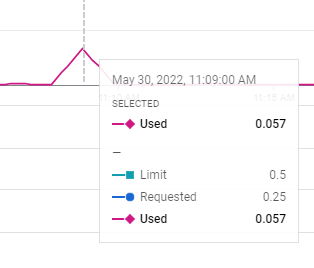
\includegraphics[width=0.5\textwidth]{resources/ch4/resource/2-cpu.png}
	\caption{Penggunaan CPU pada kasus \textbf{SI2}}
	\label{result_cpu_2}
\end{figure}

\begin{figure}[!htb]
	\centering
	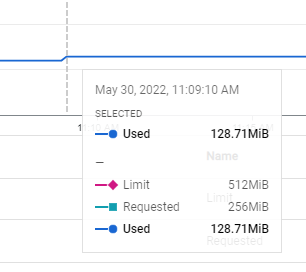
\includegraphics[width=0.5\textwidth]{resources/ch4/resource/2-mem.png}
	\caption{Penggunaan Memory pada kasus \textbf{SI2}}
	\label{result_mem_2}
\end{figure}

\pagebreak

\subsubsection{Kasus SI3}
Dari gambar \ref{result_cpu_3} dan \ref{result_mem_3} terlihat bahwa PRA Engine menggunakan \textit{resource} CPU sebanyak 0,071 vCPU dan Memory sebanyak 131,55 MiB. 

\begin{figure}[!htb]
	\centering
	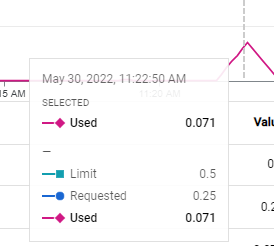
\includegraphics[width=0.5\textwidth]{resources/ch4/resource/3-cpu.png}
	\caption{Penggunaan CPU pada kasus \textbf{SI3}}
	\label{result_cpu_3}
\end{figure}

\begin{figure}[!htb]
	\centering
	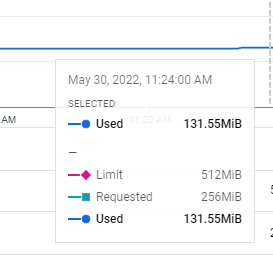
\includegraphics[width=0.5\textwidth]{resources/ch4/resource/3-mem.png}
	\caption{Penggunaan Memory pada kasus \textbf{SI3}}
	\label{result_mem_3}
\end{figure}

\pagebreak

\subsubsection{Kasus SI4}
Dari gambar \ref{result_cpu_4} dan \ref{result_mem_4} terlihat bahwa PRA Engine menggunakan \textit{resource} CPU sebanyak 0,059 vCPU dan Memory sebanyak 146,6 MiB. 

\begin{figure}[!htb]
	\centering
	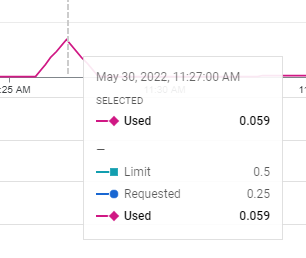
\includegraphics[width=0.5\textwidth]{resources/ch4/resource/4-cpu.png}
	\caption{Penggunaan CPU pada kasus \textbf{SI4}}
	\label{result_cpu_4}
\end{figure}

\begin{figure}[!htb]
	\centering
	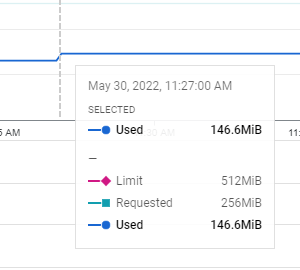
\includegraphics[width=0.5\textwidth]{resources/ch4/resource/4-mem.png}
	\caption{Penggunaan Memory pada kasus \textbf{SI4}}
	\label{result_mem_4}
\end{figure}

\pagebreak

\subsubsection{Kasus SI5}
Dari gambar \ref{result_cpu_5} dan \ref{result_mem_5} terlihat bahwa PRA Engine menggunakan \textit{resource} CPU sebanyak 0,064 vCPU dan Memory sebanyak 153,61 MiB. 

\begin{figure}[!htb]
	\centering
	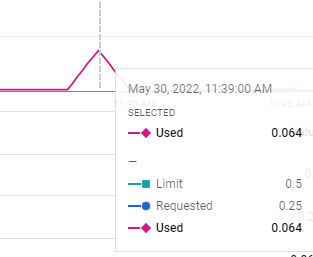
\includegraphics[width=0.5\textwidth]{resources/ch4/resource/5-cpu.png}
	\caption{Penggunaan CPU pada kasus \textbf{SI5}}
	\label{result_cpu_5}
\end{figure}

\begin{figure}[!htb]
	\centering
	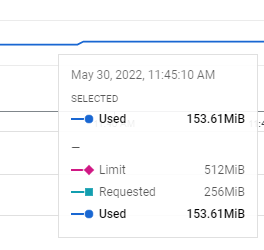
\includegraphics[width=0.5\textwidth]{resources/ch4/resource/5-mem.png}
	\caption{Penggunaan Memory pada kasus \textbf{SI5}}
	\label{result_mem_5}
\end{figure}

\pagebreak

\subsubsection{Kasus SI6}
Dari gambar \ref{result_cpu_6} dan \ref{result_mem_6} terlihat bahwa PRA Engine menggunakan \textit{resource} CPU sebanyak 0,068 vCPU dan Memory sebanyak 153,61 MiB. 

\begin{figure}[!htb]
	\centering
	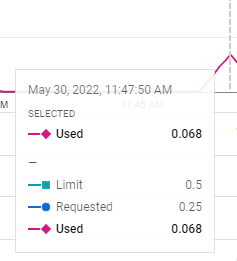
\includegraphics[width=0.5\textwidth]{resources/ch4/resource/6-cpu.png}
	\caption{Penggunaan CPU pada kasus \textbf{SI6}}
	\label{result_cpu_6}
\end{figure}

\begin{figure}[!htb]
	\centering
	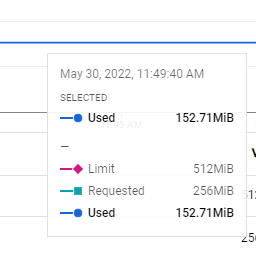
\includegraphics[width=0.5\textwidth]{resources/ch4/resource/6-mem.png}
	\caption{Penggunaan Memory pada kasus \textbf{SI6}}
	\label{result_mem_6}
\end{figure}

\pagebreak

\subsubsection{Kasus SI7}
Dari gambar \ref{result_cpu_7} dan \ref{result_mem_7} terlihat bahwa PRA Engine menggunakan \textit{resource} CPU sebanyak 0,046 vCPU dan Memory sebanyak 152,71 MiB. 

\begin{figure}[!htb]
	\centering
	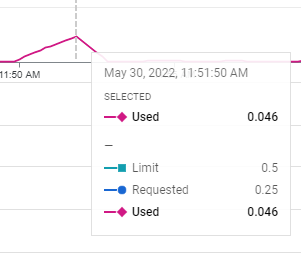
\includegraphics[width=0.5\textwidth]{resources/ch4/resource/7-cpu.png}
	\caption{Penggunaan CPU pada kasus \textbf{SI7}}
	\label{result_cpu_7}
\end{figure}

\begin{figure}[!htb]
	\centering
	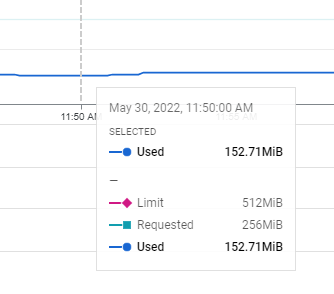
\includegraphics[width=0.5\textwidth]{resources/ch4/resource/7-mem.png}
	\caption{Penggunaan Memory pada kasus \textbf{SI7}}
	\label{result_mem_7}
\end{figure}

\pagebreak

\subsubsection{Kasus SE1}
Dari gambar \ref{result_cpu_8} dan \ref{result_mem_8} terlihat bahwa PRA Engine menggunakan \textit{resource} CPU sebanyak 0,075 vCPU dan Memory sebanyak 168,8 MiB. 

\begin{figure}[!htb]
	\centering
	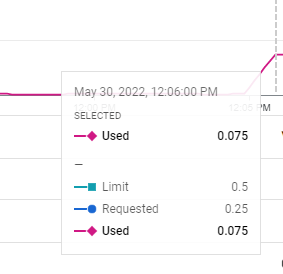
\includegraphics[width=0.5\textwidth]{resources/ch4/resource/8-cpu.png}
	\caption{Penggunaan CPU pada kasus \textbf{SE1}}
	\label{result_cpu_8}
\end{figure}

\begin{figure}[!htb]
	\centering
	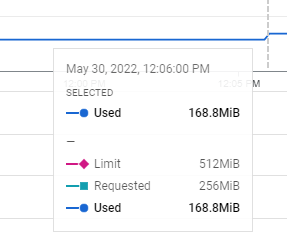
\includegraphics[width=0.5\textwidth]{resources/ch4/resource/8-mem.png}
	\caption{Penggunaan Memory pada kasus \textbf{SE1}}
	\label{result_mem_8}
\end{figure}

\pagebreak

\subsubsection{Kasus SE2}
Dari gambar \ref{result_cpu_9} dan \ref{result_mem_9} terlihat bahwa PRA Engine menggunakan \textit{resource} CPU sebanyak 0,061 vCPU dan Memory sebanyak 183,68 MiB. 

\begin{figure}[!htb]
	\centering
	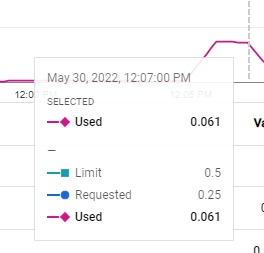
\includegraphics[width=0.5\textwidth]{resources/ch4/resource/9-cpu.png}
	\caption{Penggunaan CPU pada kasus \textbf{SE2}}
	\label{result_cpu_9}
\end{figure}

\begin{figure}[!htb]
	\centering
	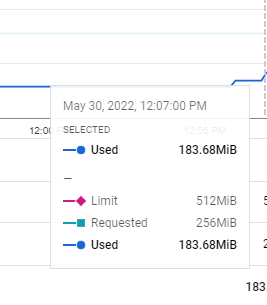
\includegraphics[width=0.5\textwidth]{resources/ch4/resource/9-mem.png}
	\caption{Penggunaan Memory pada kasus \textbf{SE2}}
	\label{result_mem_9}
\end{figure}

\pagebreak

\subsubsection{Kasus SE3}
Dari gambar \ref{result_cpu_10} dan \ref{result_mem_10} terlihat bahwa PRA Engine menggunakan \textit{resource} CPU sebanyak 0,073 vCPU dan Memory sebanyak 176,59 MiB. 

\begin{figure}[!htb]
	\centering
	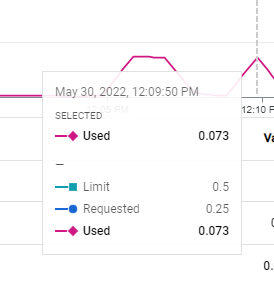
\includegraphics[width=0.5\textwidth]{resources/ch4/resource/10-cpu.png}
	\caption{Penggunaan CPU pada kasus \textbf{SE3}}
	\label{result_cpu_10}
\end{figure}

\begin{figure}[!htb]
	\centering
	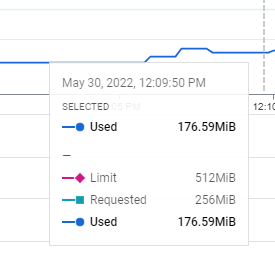
\includegraphics[width=0.5\textwidth]{resources/ch4/resource/10-mem.png}
	\caption{Penggunaan Memory pada kasus \textbf{SE3}}
	\label{result_mem_10}
\end{figure}

\pagebreak


\subsubsection{Kasus SE4}
Dari gambar \ref{result_cpu_11} dan \ref{result_mem_11} terlihat bahwa PRA Engine menggunakan \textit{resource} CPU sebanyak 0,048 vCPU dan Memory sebanyak 165,75 MiB. 

\begin{figure}[!htb]
	\centering
	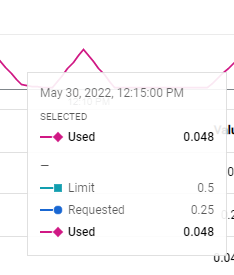
\includegraphics[width=0.5\textwidth]{resources/ch4/resource/11-cpu.png}
	\caption{Penggunaan CPU pada kasus \textbf{SE4}}
	\label{result_cpu_11}
\end{figure}

\begin{figure}[!htb]
	\centering
	\includegraphics[width=0.5\textwidth]{resources/ch4/resource/11-mem.png}
	\caption{Penggunaan Memory pada kasus \textbf{SE4}}
	\label{result_mem_11}
\end{figure}

\pagebreak

\subsubsection{Rata-rata hasil}
Dari sebelas kasus pengujian, PRA Engine rata-rata menggunakan \textit{resource} CPU sebesar 0,047 vCPU dan \textit{resource} Memory sebesar 154,412 MiB. Keseluruhan \textit{cluster} memiliki \textit{resource} sebanyak 6 vCPU dan 22,5 GiB, sehingga PRA Engine mengakibatkan \textit{overhead} CPU sebanyak 0,78 \% dan Memory sebanyak 0,67 \% kepada \textit{cluster} Kubernetes.

\subsection{Analisis Hasil Pengujian}
Dari tujuh kasus uji, kasus SI1 sampai SI7, yang menyimulasikan terjadinya regresi akibat perubahan di level kode, hanya satu kasus, yaitu kasus SI1, yang regresi tidak dapat terdeteteksi oleh PRA Engine. Selebihnya, dari enam kasus lainnya, PRA Engine dapat mendeteksi terjadinya regresi dan juga dapat menentukan kandidat operasi sumber terjadinya regresi dengan menghitung selisih \textit{latency} antara data \textit{trace} \textit{baseline} dan \textit{real-time}. 

\begin{figure}[!htb]
	\centering
	\includegraphics[width=1\textwidth]{resources/ch4/log/1-log.png}
	\caption{\textit{Log} hasil pengujian kasus SI1}
	\label{result_log_1}
\end{figure}

Gambar \ref{result_log_1} merupakan \textit{log} yang didapatkan dari kasus SI1 yang menampilkan hasil tes statistik K-S. Nilai \texttt{p-value} yang didapatkan dari hasil tes lebih besar dari nilai signifikan yaitu 0.05 dan juga nilai \texttt{statistic} lebih kecil dari nilai \texttt{critical value} sehingga hipotesis $h_{0}$ tidak dapat ditolak dan PRA Engine menginterpretasikan bahwa data \textit{latency} dari kasus SI1 berasal dari distribusi yang sama dengan data \textit{latency} \textit{baseline}. 

Dari analisis hasil kasus SI1 dapat terlihat bahwa algoritme tidak dapat mendeteksi terjadinya regresi jika tidak terdapat perbedaan signifikan antara kedua sampel data seperti pada kasus SI1 yang hanya menyimulasikan penambahan \textit{latency} sebesar 100ms pada satu buah operasi. Sementara pada kasus selanjutnya, yaitu kasus SI2 dengan penambahan \textit{latency} sebesar 250ms, PRA Engine dapat mendeteksi bahwa data \textit{latency} \textit{real-time} berasal dari distribusi yang berbeda dengan data \textit{latency} \textit{baseline} sehingga PRA Engine dapat mendeteksi terjadinya regresi.

Sementara pada kasus-kasus yang menyimulasikan perubahan dari eksternal, yaitu kasus SE1 sampai SE4, PRA Engine juga dapat mendeteksi terjadinya regresi karena algoritme dapat menentukan bahwa data \textit{latency} pada kasus-kasus tersebut berasal dari distribusi yang berbeda dari data \textit{latency} \textit{baseline}.

Dapat disimpulkan bahwa algoritme belum dapat menentukan apakah regresi yang terjadi diakibatkan oleh perubahan yang terjadi pada level aplikasi ataupun perubahan yang terjadi di luar aplikasi seperti peningkatan jumlah pengguna ataupun peningkatan \textit{load} pada sebagian operasi. Namun jika dari analisis \textit{critical path} dapat terlihat selisih \textit{latency} dari operasi yang melebihi \textit{threshold} tertentu dapat menjadi inidikasi bahwa regresi yang terjadi diakibatkan oleh perubahan di level aplikasi. Sebaliknya, jika analisis \textit{critical path} tidak dapat menentukan operasi yang menjadi kandidat penyebab regresi karena selisihnya tidak lebih besar daripada \textit{threshold}, seperti yang terlihat pada gambar \ref{result_json_8}, maka dapat menjadi indikasi bahwa regresi yang terdeteksi diakibatkan oleh perubahan yang disebabkan oleh faktor eksternal.
